\Problem{Producing a Potential Energy Graph}{\ProdPotEG}{
Below is a set of axes on which you are going to draw a potential energy curve. By doing experiments, you find the following information:
\begin{itemize}
	\item A particle with energy $ E_{1} $ oscillates between positions D and E.
	\item A particle with energy $ E_{2} $ oscillates between positions C and F.
	\item A particle with energy $ E_{3} $ oscillates between positions B and G.
	\item A particle with energy $ E_{4} $ enters from the right, bounces at A, then never returns.
\end{itemize}
Draw a potential energy curve that is consistent with this information.
}
\ProblemFig{\ProdPotEGFig}{
\centering
\if\GrayProb1
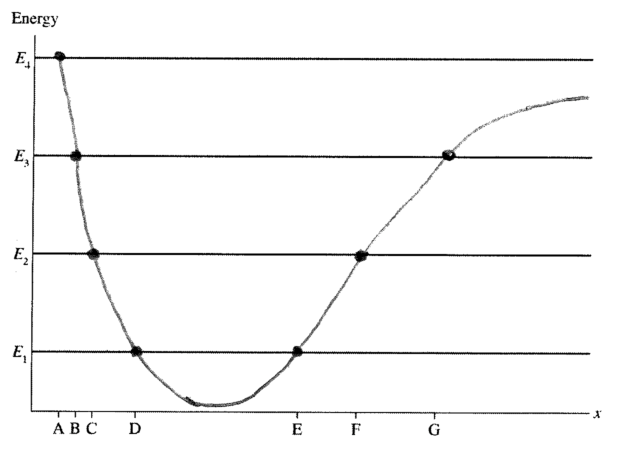
\includegraphics{\FileDepth/Activities/Producing_a_Potential_Energy_Graph/Solved_PE_Graph_with_Energies.pdf}
\else
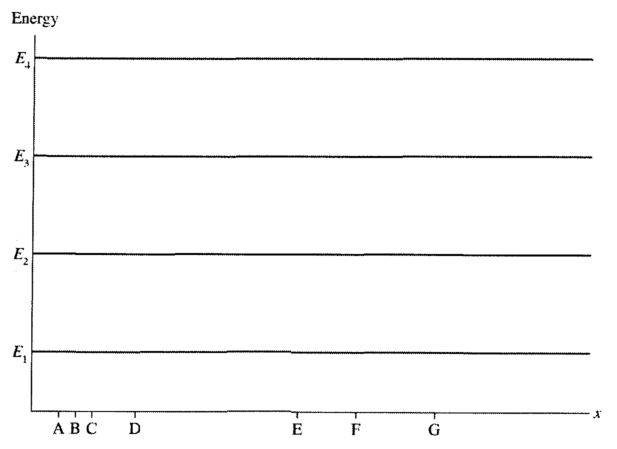
\includegraphics{\FileDepth/Activities/Producing_a_Potential_Energy_Graph/Blank_PE_Graph_with_Energies.pdf}
\fi
}
\Solution{\ProdPotEGComment}{

This is just one realization of the graph. Other solutions are possible with extra wiggles. Wherever you are at on the graph, as long as the wiggle you add does not cross above the next energy level above and create new turning points, the graph will still be correct. You may even create wiggles that cross energy levels lower than where you are at on the graph.
}